\documentclass[
	12pt,
	a4paper,
	BCOR10mm,
	%chapterprefix,
	DIV14,
	headsepline,
	%twoside,
	%openright
]{scrreprt}

\KOMAoptions{
	listof=totoc,
	bibliography=totoc,
	index=totoc
}

\usepackage[T1]{fontenc}
\usepackage[utf8]{inputenc}

\usepackage{lmodern}

\usepackage[ngerman,english]{babel}

\usepackage[toc]{appendix}
\usepackage{eurosym}
\usepackage{fancyhdr}
\usepackage{graphicx}
\usepackage[htt]{hyphenat}
\usepackage{listings}
\usepackage{amsmath}
\usepackage{microtype}
\usepackage[list=true,hypcap=true]{subcaption}
\usepackage{units}

\usepackage{varioref}
\usepackage[hidelinks]{hyperref}
\usepackage[capitalise,noabbrev]{cleveref}

\lstset{
	basicstyle=\ttfamily,
	frame=single,
	numbers=left,
	language=C,
	breaklines=true,
	breakatwhitespace=true,
	postbreak=\hbox{$\hookrightarrow$ },
	showstringspaces=false,
	tabsize=4,
	captionpos=b,
	morekeywords={gboolean,gpointer,gconstpointer,gchar,guchar,gint,guint,gshort,gushort,glong,gulong,gint8,guint8,gint16,guint16,gint32,guint32,gint64,guint64,gfloat,gdouble,gsize,gssize,goffset,gintptr,guintptr,int8_t,uint8_t,int16_t,uint16_t,int32_t,uint32_t,int64_t,uint64_t,size_t,ssize_t,off_t,intptr_t,uintptr_t,mode_t}
}

\makeatletter
\renewcommand*{\lstlistlistingname}{List of Listings}
\makeatother

\begin{document}

\begin{titlepage}
	\begin{center}
		{\titlefont\huge Programmieren einer Partikelsimulation für kurzreichweitige Interaktionen\par}

		\bigskip
		\bigskip

		{\Large Projektbericht\par}

		\bigskip
		\bigskip

		{\large Arbeitsbereich Wissenschaftliches Rechnen\\
		Fachbereich Informatik\\
		Fakultät für Mathematik, Informatik und Naturwissenschaften\\
		Universität Hamburg\par}
	\end{center}

	\vfill

	{\large\begin{tabular}{ll}
		Vorgelegt von:  & \begin{tabular}{@{}l@{}}Oliver Heidmann, \\ Benjamin Warnke\end{tabular} \\
		E-Mail-Adresse: & \begin{tabular}{@{}l@{}}\href{mailto:adresse@email.de}{adresse@email.de},\\ \href{mailto:4bwarnke@informatik.uni-hamburg.de}{4bwarnke@informatik.uni-hamburg.de}\end{tabular}\\
		Matrikelnummer: & \begin{tabular}{@{}l@{}}1234567,\\6676867\end{tabular} \\
		Studiengang:    & Informatik\\
		\\
		Betreuer:       & Philipp Neumann \\
		\\
		Hamburg, den 09.03.2017
	\end{tabular}\par}
\end{titlepage}

\chapter*{Abstract}

\thispagestyle{empty}

%TODO 
Ziel des dieses Projektes ist die Implementierung einer Partikel-Simulation für kurzreichweitige Partikel-Interaktionen mit Autotuning.

\tableofcontents

\chapter{Einleitung}
\label{Einleitung}

Bei Partikel Simulationen müssen normalerweise die Wechselwirkungen zwischen jedem möglichen Partikelpaar berechnet werden. Die Laufzeit des Programms steigt quadratisch zur Anzahl der Partikel. Dies ist besonders bei hohen Anzahlen von Partikeln kritisch für die Laufzeit. Die in diesem Projekt implementierte Partikel-Simulation ist für kurzreichweitige Interaktionen optimiert. Dadurch lassen sich die Interaktionen zwischen weit auseinanderliegenden Partikeln vernachlässigen, wodurch die Laufzeit kürzer werden kann. Es gibt verschiedene Möglichkeiten, die Interaktionen auf die kurzreichweitige Interaktion zu beschränken um das Programm zu beschleunigen. Das Problem bei diesen verschiedenen Möglichkeiten der Beschleunigung besteht darin, dass je nach Eingabe eine andere Art der Vereinfachung eine bessere Programm-Laufzeit ermöglicht. Die Besonderheit dieser Partikel Simulation liegt darin, dass das Programm zu beginn selbst entscheiden kann, welche Optimierungsstrategie für die gegebene Eingabe am sinnvollsten ist. Hieraus resultiert der Vorteil gegenüber anderen Programmen, dass die Laufzeit für jede beliebige Eingabe besonders schnell ist, und nicht nur wenn die Eingabe passend ist. Dies ist besonders dann spannend, wenn man selbst nicht sicher ist, welches verfahren für die Eingabe am besten geeignet ist, ohne selbst vorher alle Möglichkeiten einmal auszuprobieren.

\chapter{Realisierung}
\label{Realisierung}
\section{Vorgehen}

%TODO 
planung
aufteilung + zeitplan -> realität
zeiteinschätzung vs reale zeit
unerwartete schwierigkeiten

\newpage
\section{Design}
\begin{figure}[h]
	\centering
	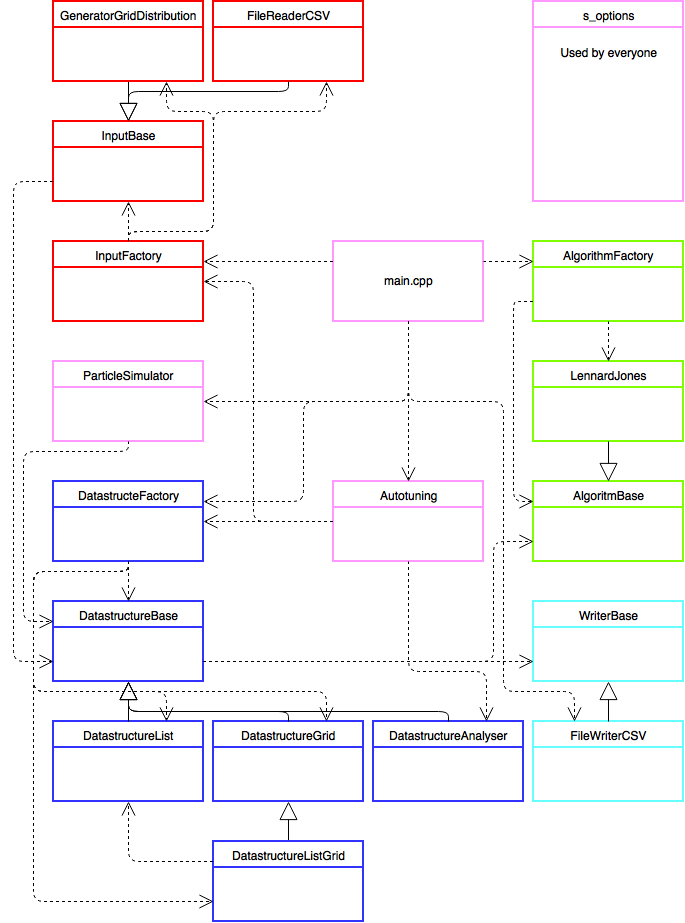
\includegraphics[height=0.6\textheight]{ClassDiagram.png}
	\caption{Klassendiagramm}
	\label{figure:Klassendiagramm}
\end{figure}
%TODO 
welche klasse tut was
für spätere programierer erklären

\section{Implementierung}

%TODO 
beschreiben der benutzung(parameter)

\section{Analyse}
\subsection{Korrektheit}
Um sicherzustellen, dass das Programm korrekte Ausgaben liefert, wurden verschiedene Arten von Test durchgeführt. Zum einen wurden einzelne Komponenten getestet, zum anderen wurde auch das Gesamtverhalten des Programms überprüft.
\begin{itemize}
	\item \textbf{unit-Tests} Um die Korrektheit von den einzelnen Komponenten des Programms zu gewährleisten wurden unit-Tests eingesetzt. Schon beim schreiben der unit-tests wurden viele Fehler gefunden und behoben. Bei späteren Refactoring-Maßnahmen wurden durch diese Testfälle viele neue Fehler verhindert.
	\item \textbf{Energieerhaltung} Aus dem Physikalischen Gesetz 'Aktion gleich Reaktion' ergibt sich, dass die Energie in einem geschlossenen System immer erhalten belieben muss. Eingebaute Funktionen im Programm ermöglichen die Ausgabe der aktuellen Energie im System, sodass leicht überprüft werden kann, ob die Energie in einem Akzeptablen Rahmen beleibt. Durch Rechenungenauigkeiten ist es sehr unwahrscheinlich, dass die Energie exakt gleich beleibt.
	\item \textbf{Visualisierung} Durch Visualisieren der Ausgabedaten wurde auch das fertige Ergebnis stichprobenartig überprüft. Bei den getesteten Parametern verhielt sich das Programm wie erwartet.
\end{itemize}

\subsection{Laufzeit}
Die Laufzeit des Programmes hängt von der Anzahl der zu simulierenden Partikel ab. Bei kurzreichweitigen Interaktionen kann man die Laufzeitabschätzung mit $p\cdot\frac{r^3}{V}\sim O\left(1\right)$ vereinfachen (siehe Tabelle \ref{table:Laufzeitvergleich}).\\
\begin{table}[h]
	\centering
	\begin{tabular}{c|l|l|l|l}
		&Basic& Nachbar-Listen & Linked-Cells & Kombination \\
		\hline
		\begin{tabular}{@{}c@{}}Aufbau \\ (Linked-Cells)\end{tabular} &-& - & $\Theta\left(p\right)$& $\Theta\left(p\right)$\\
		\hline
		\begin{tabular}{@{}c@{}}Aufbau \\ (Nachbar-Listen)\end{tabular}&-& $\Theta\left(p^2\right)$ & - & \begin{tabular}{@{}l@{}}$O\left(p^2\cdot \frac{27 \cdot r^3}{V}\right)$ \\ $\sim O\left(p\cdot 27\right)$\end{tabular} \\
		\hline
		Iteration& $\Theta\left(p^2\right)$&\begin{tabular}{@{}l@{}}$O\left(p^2\cdot \frac{\frac{4}{3}\pi\cdot r^3}{V}\right)$\\$\sim O\left(p\cdot \frac{4}{3}\pi\right)$\end{tabular} &\begin{tabular}{@{}l@{}}$O\left(p^2\cdot \frac{27 \cdot r^3}{V}\right)$\\$\sim O\left(p\cdot 27\right)$ \end{tabular}& \begin{tabular}{@{}l@{}}$O\left(p^2\cdot \frac{\frac{4}{3}\pi\cdot r^3}{V}\right)$\\$\sim O\left(p\cdot \frac{4}{3}\pi\right)$ \end{tabular}\\
	\end{tabular}
	\caption{Laufzeitvergleich der Datenstrukturen}
	\label{table:Laufzeitvergleich}
\end{table}\\
Je nachdem, welches Verfahren gewählt wird, ist die Laufzeit unterschiedlich. Bei der Variante bei der nur Nachbar-Listen verwendet werden ist der Aufwand diese Listen aufzubauen Quadratisch zur Anzahl der Partikel. Dies ist so ungünstig, dass es nicht empfehlenswert ist, diese Variante zu Benutzen. Die Linked-Cells-Variante benötigt wenig Zeit um die Datenstruktur aufzubauen, dafür aber wird pro Iteration viel Zeit benötigt. Die Kombinierte Variante benötigt mittelmäßig viel Zeit für den Aufbau der Datenstruktur kosten, und nur Minimale Zeit pro Iteration.

Damit das Auto-tuning entscheiden kann, welche Variante verwendet werden soll, muss das Programm abschätzen können, wie oft die Datenstruktur neu gebaut werden muss. Es gibt mehrere Faktoren, die einen Einfluss auf die Häufigkeit des Neubauen der Datenstruktur haben.
\begin{itemize}
	\item \textbf{Dichte} Wenn die Partikel dichter aneinander liegen, dann werden durch die nur Zellen-basierte Optimierung zu wenig Partikel frühzeitig für die Berechnung eliminiert, was zu einer stärkeren Laufzeiterhöhung führt, als wenn die Kombinierte Variante verwendet werden würde.
	%\item \textbf{Volumen} wie Dichte ?!?
	\item \textbf{Anzahl} Wenn die Anzahl sehr gering ist, dann ist die Laufzeit des naiven Algorithmus ohne Optimierung kürzer, als eine der Optimierten Varianten, da der Naive Algorithmus nur sehr kleine Konstanten hat.
	\item \textbf{cut-off} Je größer der cut-off Radius gewählt wird, desto mehr Partikel befinden sich in der Nachbarschaft. Die Zellen werden hierdurch größer. Wenn der cut-off Radius relativ groß ist, dann ist der Listenaufbau auch in der Kombinierten Variante Laufzeit-intensiv, wodurch die nur Zellen basierte Variante im Vorteil ist. Da dieses Programm sich auf kurzreichweitige Interaktionen fokussiert, werden keine sehr großen cut-off-Radien auftreten.
	\item \textbf{cut-off Faktor} Je mehr Spielraum auf den cut-off hinzugefügt wird, desto seltener müssen die Datenstrukturen neu aufgebaut werden. Dies geht allerdings auch sehr zulasten der Laufzeit, die in den Iterationen gebraucht wird.
	\item \textbf{Startgeschwindigkeit} Je schneller sich die Partikel sich bewegen, desto schneller wird der cut-off Bereich verlassen. Hieraus folgt, dass die Datenstruktur besonders oft neu aufgebaut werden muss. Hier ist die nur Zellen basierte im Vorteil.
	\item \textbf{Startanordnung} Je nachdem wie die Partikel bei Programmstart angeordnet sind ergeben sich andere Effekte. Zum Beispiel wäre es möglich, dass sich zu beginn alle Partikel in einem kleinem Bereich des zu simulierenden Raum aufhalten. Hieraus folgt, dass einige Zellen sehr viel mehr Partikel enthalten als andere. Für die gemischte Variante würde dies Bedeuten, dass die zweite Aufbauphase in einigen Zellen sehr viel Laufzeit benötigt.
\end{itemize}
\subsection{Auto-tuning}
%TODO 
\begin{itemize}
	\item \textbf{c} $\rightarrow$ cut-off-radius
	\item \textbf{f} $\rightarrow$ cut-off-radius-factor
	\item \textbf{s} $\rightarrow$ start-speed
\end{itemize}

\begin{align*}
2\cdot s < c \cdot (f - 1) - 1
\end{align*}

\begin{itemize}
	\item \textbf{true} $\rightarrow$ linked-cells+verlet-list
	\item \textbf{false} $\rightarrow$ linked-cells
\end{itemize}
\chapter{Zusammenfassung}
\label{Zusammenfassung}

%TODO 

\chapter{Literatur}
\label{Literatur}

%TODO 

\chapter{Anhang}
\label{Anhang}

Verwendete Bibliotheken und Programme zum ausführen des Programms
\begin{itemize}
	\item Boost
	\begin{itemize}
		\item unit-tests
	\end{itemize}
	\item CMake 
	\item Make
	\item clang-format
	\item paraview
	\begin{itemize}
		\item Visualisierung der Ausgabe
	\end{itemize}
	\item lcov
	\begin{itemize}
		\item Testabdeckung ermitteln und visualisieren
	\end{itemize}
	\item slurm
	\begin{itemize}
		\item Messtabellen berechnen
	\end{itemize}
	\item doxygen
	\begin{itemize}
		\item Dokumentation des Quelltextes
	\end{itemize}
	\item latex
	\begin{itemize}
		\item dieses Dokument
		\item Präsentationen
	\end{itemize}
\end{itemize}




\end{document}
